\section{Fundamentals}
\label{sec:fundamentals}
Storing the range values of a given function $\Fx$ for a discretized domain can help to avoid a computationally expensive 
polynomial approximation of $\Fx$. %can be just replaced by a search routine of the range value of $x$ in a lookup table.
Unfortunately, this approach is impractical in case the given approximation error demands fine quantization of the domain. 
Indeed, the table size required to store the range values grows exponentially with the bit-width of $x$.
E.g., if the bit-width for quantization of $x$ is 8 bits, the size of the lookup table is $2^8 = 255$.
However, if the bit-width of $x$ is 32, the lookup table contains $2^{32}=4,294,967,296$ entries, thus resulting in a memory footprint of 16 GB.
Consequently, this method cannot be applied for 
resource-constrained devices such as \acp{FPGA} due to the limited amount of available memory and other hardware resources. 
As a solution, the combination of tabular function representation and polynomial interpolation has emerged as a widespread technique for function approximation on \acp{FPGA}~\cite{luttab}. 
Instead of storing all the range values of $\Fx$ for a given quantization of $x$, a more efficient approach is to use a coarser quantization of $x$ and perform polynomial approximation in between two adjacent points called breakpoints in the following. 
In \cite{luttab}, it is proposed to use a degree $n$ polynomial $p(x)$ as follows:
\begin{equation}
p(x)=a_0+a_1x+\ldots+a_nx^n
\label{eq:pol}
\end{equation}
Here, $a_i: 0 \leq i \leq n$ denotes the coefficients of the approximating polynomial $p(x)$.
Accordingly, the number of entries of the table can be reduced. 
Still, this requires to store the $n+1$ additional coefficients of each polynomial in between two adjacent breakpoints.\\
In the rest of this paper, we consider piecewise linear interpolation to avoid the increased computational complexities and memory requirements of higher degree polynomials. In general, breakpoints do not have to be located equidistantly. In this case, linear interpolation can be performed using \cref{eq:linEq}. For example, the set of $k+1$ breakpoints is denoted as $X = \{ x_0, x_1, \ldots, x_k\}$. $Y$ represents the range value of $\Fx$ for $X$ as domain $Y= \{f(x_0),f(x_1),\ldots, f(x_k) \} = \{y_0, y_1, \ldots, y_k\}$. The first and last breakpoints $\{x_0, x_k=\UpperBound\} \in X$ enclose the interval of approximation. \cref{fig:interpolation} illustrates the calculation of $\Fx$ for any given $x \in {\bf R}$. If $x$ matches with any value in $X$, the result can be directly retrieved from a table storing the values of $Y$. Otherwise, the first step is to find the closest breakpoints $x_i$ and $x_{i+1}$ of the input. Their corresponding range values $y_i$ and $y_{i+1}$ are then looked up. Finally, the value of $\Fx$ is computed according to \cref{eq:linEq}.
\begin{equation}
\RangeBreakpoint{ } = \RangeBreakpoint{i} + \dfrac{\Breakpoint{ }-\Breakpoint{i}}{\Breakpoint{i+1}-\Breakpoint{i}}(\RangeBreakpoint{i+1}-\RangeBreakpoint{i})
\label{eq:linEq}
\end{equation}
\begin{figure}[t]
  \centering
  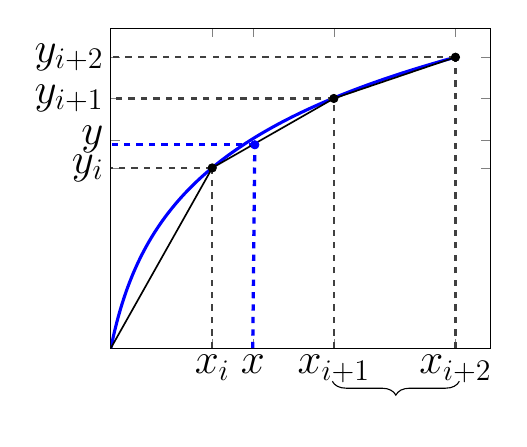
\begin{tikzpicture}[scale=0.75]
    \begin{axis}[
        width=8cm,
        height=7cm,
        xmin=1,
        ymin=0,
        %xmax=6.5,
        %ymax=5.5,
        xtick = {6,8,12,18},
        ytick = {1.79,2.07,2.48,2.89},
        xticklabels={\huge $x_i$,\huge $x$,\huge $x_{i+1}$,\huge$x_{i+2}$},
        yticklabels={\huge $y_i$ ,\huge $y$,\huge $y_{i+1}$,\huge$y_{i+2}$},
        ]

          \addplot[black,mark=none,line width=1.5pt,domain=1:18,samples=400,color=blue]  {ln(x)} node[above left,yshift=-0.5cm,xshift=-4.5cm] {};

      \addplot[only marks, black]  coordinates {(6,1.79) (12,2.48) (18,2.89)};
      \addplot[only marks, blue]  coordinates  {(8.1,2.02)};

      \draw[very thick, dashed,draw=black!75] (axis cs:6,0) -- (axis cs:6,1.79);
      \draw[very thick, dashed,draw=black!75] (axis cs:6,1.79) -- (axis cs:0,1.79);

      \draw[ultra thick, dashed,draw=blue] (axis cs:8,0) -- (axis cs:8.1,2.02);
      \draw[ultra thick, dashed,draw=blue] (axis cs:8.1,2.02) -- (axis cs:0,2.02);
          
      \draw[very thick, dashed,draw=black!75] (axis cs:12,0) -- (axis cs:12,2.48);
      \draw[very thick, dashed,draw=black!75] (axis cs:12,2.48) -- (axis cs:0,2.48);
          
      \draw[very thick, dashed,draw=black!75] (axis cs:18,0) -- (axis cs:18,2.89);
      \draw[very thick, dashed,draw=black!75] (axis cs:18,2.89) -- (axis cs:0,2.89);
          
      \draw[thick,draw=black] (axis cs:1,0) -- (axis cs:6,1.79);
      \draw[thick,draw=black] (axis cs:6,1.79) -- (axis cs:12,2.48);
      %\draw[thick,draw=black] (axis cs:8,2.07) -- (axis cs:12,2.48);                                                    
      \draw[thick,draw=black] (axis cs:12,2.48) -- (axis cs:18,2.89);                                                   
      
    \end{axis}

\draw [decorate,decoration={brace,amplitude=5pt,mirror,raise=4pt},yshift=0pt] (3.75,-0.375) -- (5.9,-0.375) node [black,midway,yshift=-0.5cm]{$\Spacing{}$};
  \end{tikzpicture}
  \caption{\label{fig:interpolation} Piecewise linear interpolation in between two breakpoints $x_i$ and $x_{i+1}$.}
\end{figure}


If $x_{i+1}-x_i$ is not constant $\forall i \in \{0,1,\hdots,k\}$, then the enclosing breakpoints can only be located by a search method. 
To this end, the number of comparisons performed grows with the number of breakpoints $k$. This can be avoided by even sampling of the interval $[\LowerBound, \UpperBound)$. Now, when defining a uniform spacing $\Spacing{ }=(x_{i+1}-x_i)>0$ between two breakpoints, it is possible to determine the index $\IndexLocation$ describing the interval $[\Breakpoint{i}, \Breakpoint{i+1})$ that includes $\Breakpoint{}$ as follows:
\begin{equation}\label{eq:even_space}
   \IndexLocation = \bigg\lfloor \frac{(\Breakpoint{}-\Breakpoint{0})}{\Spacing{ }}\bigg \rfloor
\end{equation}
Here, only the first value $\Breakpoint{0}$ and the spacing $\Spacing{ }$ are required to calculate $\IndexLocation$.
Finally, with $x_i = x_0 + i \cdot \delta$, \cref{eq:linEq} can be re-written to only use the points in $\SetRangeBreakpoints$, $\Breakpoint{0}$, the location $\IndexLocation$ according to \cref{eq:even_space} and the spacing $\Spacing{}$:
%
\begin{equation}\label{eq:2pt_line_even}
   \RangeBreakpoint{}=
   \RangeBreakpoint{i}+\frac{\Breakpoint{}-(\Breakpoint{0} + \IndexLocation \cdot \Spacing{})}{\Spacing{}}(\RangeBreakpoint{i+1}-\RangeBreakpoint{i})%& \text{if } \Breakpoint{0} \leq \Breakpoint{} \leq \Breakpoint{k}\\
\end{equation}
Thus, the function approximation can be achieved just by storing the $k+1$ range values of $X$. 
Henceforth, we only consider equidistant spacing between two breakpoints. 
The required memory footprint is referred to as $\MemF$ in the following sections.
For the above linear interpolation scheme, we obtain a memory footprint $\MemF$ of:
\begin{equation}
\MemF=k+1
\label{eq:refEquation}
\end{equation}
